\documentclass[memoire.tex]{subfiles}

\chapter{Les architectures Big Data}

Une architecture Big Data est un regroupement d'outils permettant de gérer des données de leurs ingestion à leurs mise en valeur via des analyses.
Il faut savoir qu'il existe plusieurs architectures dans le domaine du Big Data, et qu'elles répondent à des besoins différents. Nous allons nous intéresser aux deux architectures les plus importantes, étant donné que les autres sont des dérivées des deux architectures principales. Avant de voir en détail ces deux architectures, nous allons voir de manière plus générale les différents composants qui peuvent se retrouver dans des architectures Big Data~\cite{ARCH_DATA}\cite{BIGDATA_OVERALL}.
Les différents composants pouvant se retrouver dans une architecture Big Data sont illustrés sur la figure \ref{composants-architecture-big-data}.

\begin{figure}[!h]
	\centering 
	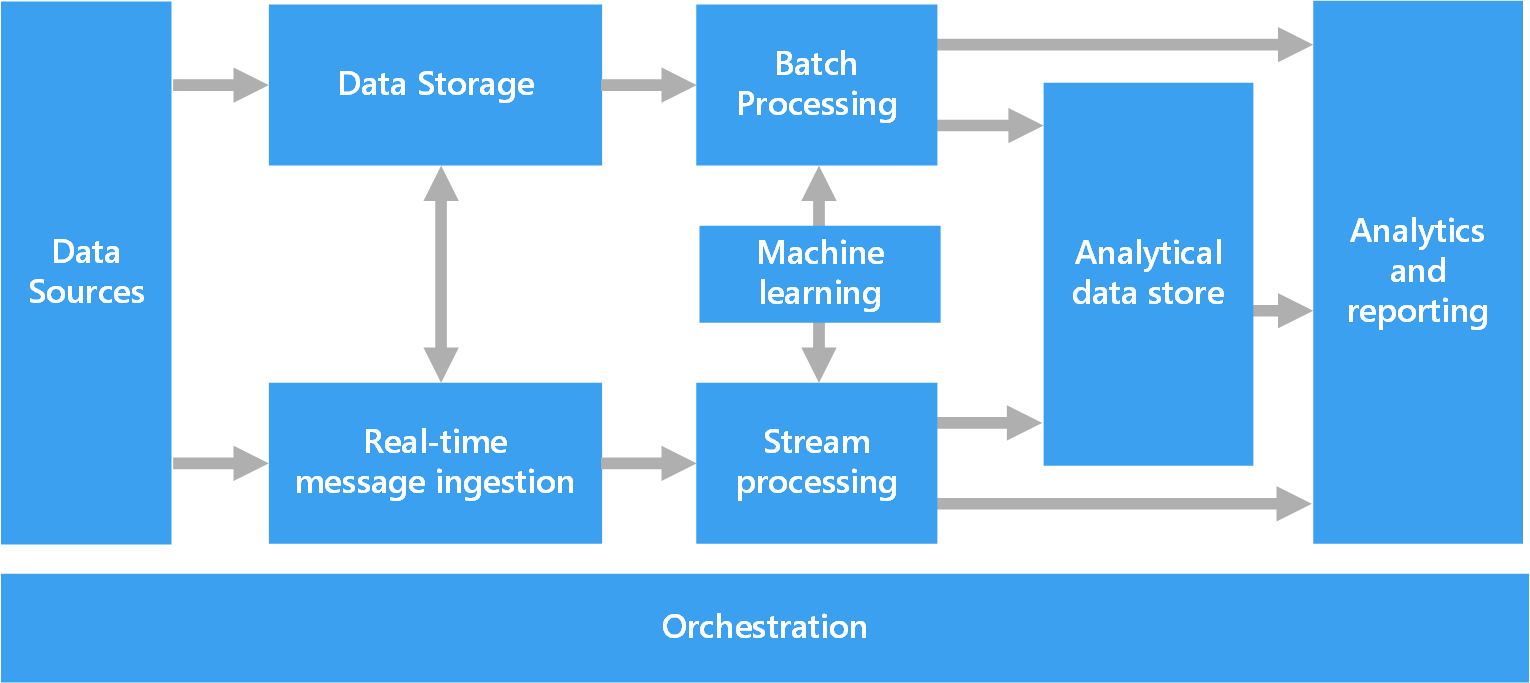
\includegraphics[scale=0.58]{img/big-data-comp.png}
	\caption{Composants d'une architecture Big Data}
	\label{composants-architecture-big-data}
\end{figure}

Nous allons maintenant détailler le rôle de chaque composant présenté dans le digramme ci dessus.

\begin{itemize}
\item \textbf{Source de données :} N'importe quelle solution Big Data a besoin d'une source de donnée en entrée. Voici quelques exemple de données qui peuvent être utilisée dans une architecture Big Data
\begin{itemize}
\item Des données issues de bases de données relationnelles.
\item Des fichiers statiques produits par des applications, des fichiers de logs par exemple.
\item Des sources de données en temps réel, par exemple des données de capteurs récupérés via des appareils IoTs.
\end{itemize}

\item \textbf{Ingestion des données :} La solution doit être capable d'aller chercher directement les données dans les différentes sources. Il est possible que les données soient directement envoyées dans la chaîne de traitement des données, mais c'est rarement le cas. Afin d'aller récupérer les données à la source, il y a plusieurs solutions. On peut écrire un programme permettant d'extraire les données. Cette solution est la plus efficace si le programme répond bien aux contraintes du Big Data, c'est à dire, il faut qu'il soit le plus réactif possible et le plus facilement adaptable aux flux de données entrant (Architecture réactive {\ref{a:architecture-reactive}}). La seconde solution la solution la plus simple, est l'utilisation d'un ETL (Extract Transform Load). C'est un outil graphique permettant de configurer l'extraction des données et leurs insertions dans la chaîne de traitements ou dans la solution de stockage. Néanmoins, cette solution est plus gourmande que l'écriture d'un programme car elle doit être capable de gérer énormément de sources et d'opérations différentes.

\item \textbf{Traitement par lot :} Les jeux de données étant trop lourd lors d'un traitement par lots, il est nécessaire de pouvoir exécuter une tâche de traitement de longue durée afin de filtrer, agréger et préparer les données en vue de leur analyse. En général, ce genre de traitement implique une lecture de fichier source et une écriture dans des nouveaux fichiers. Le traitement des données peut s'effectuer par des programmes java, scala ou Python ou encore via des outils spécialisé comme MapReduce ou Spark.  

\item \textbf{Ingestion des données en temps réel : } Si la solution doit interagir avec des sources de données en temps réel, l'architecture doit impérativement implémenter un moyen de récupérer ces données et de les stocker temporairement dans une file d'attente afin de pouvoir les temporiser. Cela permet d'éviter la perte de données entrante, et permet d'envoyer les données à la solution de traitement quand elle est disponible et de ne pas la surcharger. Généralement on utilise des messages brokers pour ce genre de tâches.  

\item \textbf{Traitement de flux :} Une fois les données récupérées, elles doivent être filtrées, agrégées puis préparer pour l'analyse. le traitement est similaire au traitement par lot, seul les outils sont différents, car ils doivent être capable de gérer le traitements en temps réel.

\item \textbf{Stockage des données :} Une solution de stockage de données est indispensable dans le cas de traitement des données par lot ({\ref{a:traitement-donnees-batch}}), et peut s'avérer utile lors de traitements des données en temps réel ({\ref{a:traitement-donnees-real-time}}) si l'on souhaite conserver les données reçues en plus de les traiter. Le deuxième cas ou un stockage de donnée peut être utile pour le traitement en temps réel, est si l'on a besoin d'agréger des données statiques avec les données en temps réel. Ces solutions de stockage doivent être capables de gérer divers formats de données, et surtout ils doivent être distribués ({\ref{a:architecture-repartie}}).

\item \textbf{Gouvernance des données :} La gouvernance des données correspond à l'ensemble des procédures mises en place afin d'encadrer la collecte des données ainsi que leur utilisation. La gouvernance des données comprend quatre dimensions. La disponibilité des données, l’utilisabilité des données, l'intégrité des données et la sécurité des données.

\item \textbf{Requêtage : } Afin de pouvoir fournir les données stockées aux outils d'analyse et de visualisation, l'utilisation d'un outil de requetâge peut être requis. Dans certains cas votre base de données et votre outil de visualisation communiqueront directement entre eux, mais dans d'autres cas vous aurez besoin d'utiliser un outil de requetâge afin de fournir les données au bon format et de pouvoir faire une sélection des données à envoyer à l'outil.

\item \textbf{Analyse et visualisation des données :} La dernière étape dans une architecture Big Data est la visualisation/analyse des données. La plupart des solutions Big Data ont pour but de faire de la valorisation de données et de fournir au minimum une visualisation des données et au mieux d'effectuer des analyses dessus. Cela peut se faire par l'écriture de rapport ou bien par application d'algorithme afin de détecter et de montrer différentes corrélations entre des données par exemple. Le but principal est d'avoir une visualisation intelligente et facilement compréhensible de données étant à la base illisible par l'homme.

\item \textbf{Orchestration : } La majorité des solutions Big Data consistent a effectuer des traitements de données répétés, ayant pour but de transformer les données sources puis de les stocker ou bien les envoyer directement à un outil d'analyse ou de visualisation des données. Il est donc important d'avoir un outil permettant de paramétrer les différentes actions que l'on souhaite effectuer sur nos données.

\end{itemize}

Comme on peut le voir une architecture Big Data possède beaucoup de catégorie, et l'on constate qu'une catégorie existe sous 2 formes, le traitement des données. Les deux architectures différentes sont justement sont tournées sur cette catégorie, et proposent chacune une vision différente du traitement des données. Ces deux architectures sont l'architecture Lambda et l'architecture Kappa~\cite{LAMBDA_KAPPA}\cite{BIGDATA_OVERALL}\cite{LAMBDA_KAPPA2}.

\section{Architecture Lambda}

L'architecture Lambda est une technique de traitement de données capable de traiter efficacement une grande quantité de donnée. L'efficacité de cette architecture provient d'un débit accru, une latence réduite et d'erreurs négligeables. Cela mène jusqu'à des applications pratiquement en temps réel. Dans le domaine du machine learning ({\ref{a:machine-learning}}), cela permettrait aux développeurs de définir des règles delta\footnote{La règle Delta est une règle d'apprentissage de la descente sur gradient permettant de mettre à jour les poids des entrées des neurones artificiels dans un réseau de neurones à une seule couche} sous la forme code logique ou de traitement de langage naturel avec des modèles de traitement de données basés sur des évènements afin d'obtenir de la robustesse, de l'automatisation et d'améliorer la qualité des données. Pour faire simple, toute modification de l'état des données est un événement pour le système, et il est possible de répondre à cet évènement via l'exécution d'une commande ou d'une procédure delta.

La récupération d'évènements est un concept qui consiste à utiliser les évènements afin d'effectuer des prévisions ou bien stocker les changements effectués sur le système en temps réel. par exemple, une personne qui interagit sur un site de réseau social va provoquer des évènements lors du chargement d'une page, de l'ajout en favoris d'un post, ou bien lors d'une demande d'ajout en ami. Ces événements peuvent être stockés en base de données ou bien traités afin d'enrichir des données déjà présentent.

Le traitement des données traite les flux d'évènements, ces événements sont stockés dans un système de données en direct. L'architecture Lambda permet le traitement des données en introduisant trois couches distinctes : 

\begin{itemize}
\item \textbf{Batch Layer}, couche de traitement par lots.
\item \textbf{Speed Layer/Stream Layer}, couche de traitement de flux
\item \textbf{Serving Layer}, couche de service.
\end{itemize}

\subsection*{Batch Layer}

Les données arrive constamment comme un flux vers le système de données. Tout nouveau flux de données entrant dans la couche de traitements par lots est calculé et traité sur un lac de données\footnote{Un lac de données (en anglais Data Lake) est une méthode de stockage des données utilisée par le big data. Ces données sont gardées dans leurs formats originaux ou sont très peu transformées.}. 

\subsection*{Speed Layer}

La couche vitesse se sert des résultats fournis par la couche de traitement par lots. Les flux de données entrant peuvent provenir de source extérieures (Ex: appareils IoT), ou bien d'événement qui ont été crée lors du traitement des données sur la couche de traitement par lots. Le second cas est spécialement vrai si l'on veut effectuer du machine learning ({\ref{a:machine-learning}}), afin de faire de la prédiction sur les prochaines données qui vont arriver. Comme son nom l'indique, la couche vitesse a une faible latence car elle ne traite que des données en temps réel contrairement à la couche de traitements par lots.

\subsection*{Serving Layer}

Les sorties de la couche de traitement par lots sont sous la forme de vues par lots, et celles de la couche vitesse sont sous la forme de vues en quasi temps réel. Ces vues sont transmises à la couche de service, qui va utiliser ces données afin de stocker ces vues et donc les rendre accessibles au client qui va les exploiter à l'aide d'outil d'analyse et de visualisation.

$\ $\\

la figure \ref{lambda}, représente un diagramme basique de ce à quoi ressemble le modèle de l'architecture lambda. 

\begin{figure}[!h]
	\centering 
	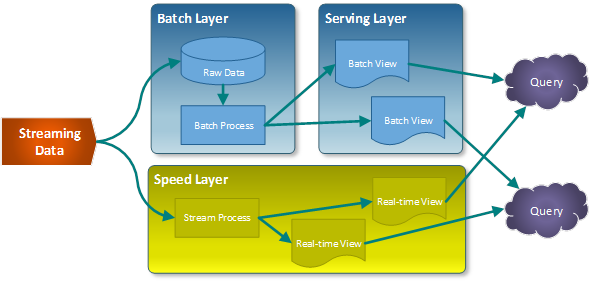
\includegraphics[scale=0.33]{img/lambda.png}
	\caption{Schéma de l'architecture Lambda}
	\label{lambda}
\end{figure}

Traduisons ce fonctionnement en une equation fonctionnelle qui définit toute requête dans le domaine du Big Data. Les symboles utilisés dans cette équation sont connus sous le nom de "Lambda" et c'est de la que cette architecture s'est vu ce nom attribué.

\[
 \text{requête} = \lambda (\text{Données complètes}) = \lambda (\text{Données temps réel}) \times \lambda (\text{Donées stockées})
\]

Cette équation signifie que toutes les requêtes relatives aux données peuvent être traitées dans l'architecture lambda en combinant les résultats du stockage historique issue tu traitement par lots et des données en temps réel.

\subsection*{Applications de l'architecture Lambda}

L'architecture Lambda peut être déployé dans les cas suivants :

\begin{itemize}
\item Le résultat des requêtes des utilisateurs, ne doit être calculé que lorsque que les requêtes sont émises (Pas de système de cache du résultat des requêtes).
\item Les réponses doivent être rapide et le système doit être capable de gérer diverses mises à jour sous la forme de nouveau flux de données.
\item Aucun des enregistrements stockés ne doit être effacé, mais l'ajout et la modification d'enregistrement doit être possible.
\end{itemize}

L'architecture Lambda peut être considéré comme une architecture de traitement de données en temps quasi réel. Comme nous l'avons mentionné précédemment, elle est tolérante aux pannes et évolutive. Elle possède une couche de traitements par lots et une couche vitesse de traitements en temps réel. Et elle garantit un stockage permanent des données. Cette architecture est utilisé par des entreprises comme Twitter, Netflix et Yahoo pour répondre aux normes de qualité de service.

\subsection*{Avantages et inconvénients de l'architecture Lambda}

Nous allons maintenant voir à partir de tout ce qu'on a vu de cette architecture, quel sont ses avantages et inconvénients.

\subsubsection*{Avantages}

\begin{itemize}
\item La couche de traitement par lots gère les données historiques avec un stockage distribué à tolérance de pannes, ce qui réduit les risques d'erreurs, même en cas de panne du système.
\item Les données fournis au client sont les plus fraiches possible.
\item Architecture à tolérance de pannes et évolutive pour le traitement des données.
\end{itemize}

\subsubsection*{Inconvénients}

\begin{itemize}
\item La logique est implémentée deux fois (couche vitesse et couche de traitement par lots).
\item Le fait de retraiter chaque traitement par lots n'est pas utile dans tous les cas.
\item Il existe des solutions plus simple lorsque le besoin n'est pas complexe.
\end{itemize}

\section{Architecture Kappa}

En 2014, Jay Kreps a entamé une discussion au cours de laquelle il a souligné certaines divergences dans l'architecture Lambda. L'architecture Kappa est née en réaction à la complexité de l'architecture Lambda, notamment avec la division du traitement par lots et du traitement en temps réel.

L'architecture Kappa ne peut en aucun cas être considérée comme un substitut de l'architecture Lambda. Au contraire, elle doit être considérée comme une alternative à celle-ci, spécifiquement dans les cas ou la couche de traitement pas lots n'est pas au premier plan. La figure \ref{Kappa} présente le fonctionnement de l'architecture Kappa.

\begin{figure}[!h]
	\centering 
	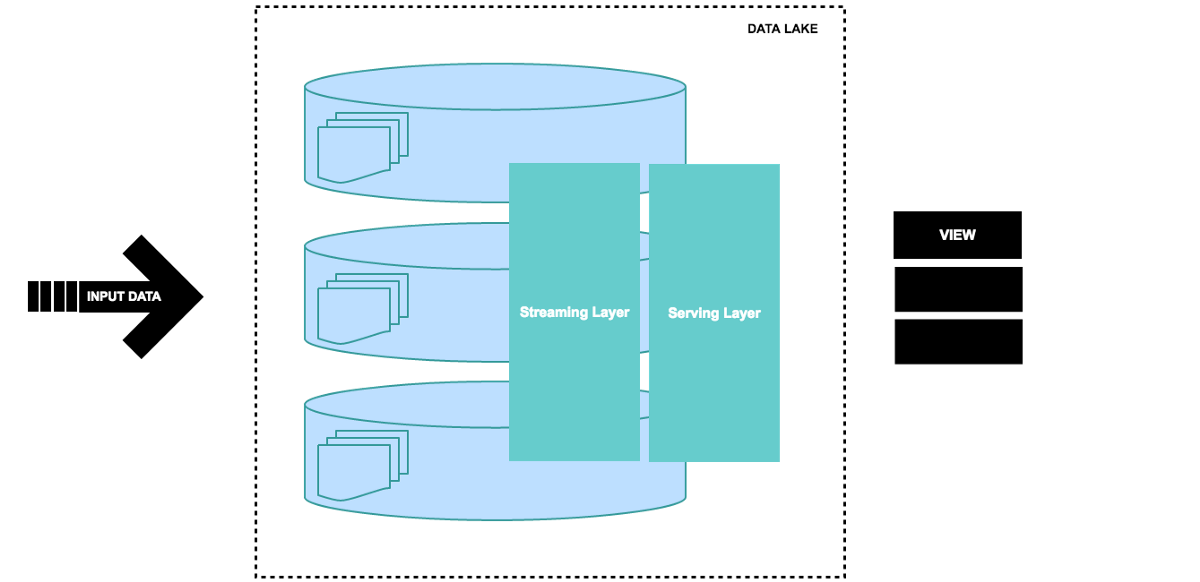
\includegraphics[scale=0.33]{img/kappa.png}
	\caption{Schéma de l'architecture Kappa}
	\label{Kappa}
\end{figure}

Traduisons le fonctionnement du traitement dans cette architecture en une équation fonctionnelle qui définit toute requête dans le domaine du Big Data.

\[
 \text{requête} = \kappa (\text{Nouvelles données}) = \kappa (\text{Flux de données en temps réel})
\]

Cette équation montre que toutes les requêtes peuvent être traités par l'application de la fonction kappa au flux de données en temps réel sur la couche de service.

\subsection*{Applications de l'architecture Kappa}

L'architecture Kappa peut être déployé dans les cas suivants :

\begin{itemize}
\item Plusieurs événements ou requêtes sont stockés dans une file d'attente avant d'être traités traités un par un.
\item L'ordre des évènements n'est pas prédéfini, et la couche de traitement de données en temps réel doit être en mesure d'interagir avec le système de stockage n'importe quand.
\item Afin de traiter des téraoctets de données, il est nécessaire que chaque nœud soit hautement disponible, résilient et supporte la réplication.
\end{itemize}

L'architecture Kappa est utilisé par des entreprises comme Linkedin.

\subsection*{Avantages et inconvénients de l'architecture Kappa}

Nous allons maintenant voir à partir de tout ce qu'on a vu de cette architecture, quel sont ses avantages et inconvénients.

\subsubsection*{Avantages}

\begin{itemize}
\item Le retraitement des données est requis uniquement lorsque le code est modifié.
\item Solution moins complexe que l'architecture Lambda.
\item Moins de ressources requise étant que le traitement se fait en temps réel.
\end{itemize}

\subsubsection*{Inconvénients}

\begin{itemize}
\item Pas de séparation entre les besoins (Temps réel et traitements par lots).
\item L'absence de couche de traitement par lots peut entraîner des erreurs lors du traitement des données ou lors de la mise à jour de la base de données.
\end{itemize}

$\ $\\
$\ $\\

Pour conclure sur ces deux architectures, l'architecture Lambda est beaucoup plus complète que l'architecture Kappa mais cela au prix d'une complexité accrue. De nombreux cas d'utilisation en temps réel conviendront parfaitement à une architecture Lambda. On ne peut pas en dire autant de l'architecture Kappa. Dans des cas où le traitement des données par lots et en temps réel sont similaire, ou bien, si le but est principalement de fournir des données métiers aux clients, l'utilisation de l'architecture Kappa est une bonne solution. Par contre dans les cas où les traitements de données en temps réel et par lots sont complètement différents ou bien si vous avez besoin d'utiliser des modèles d'apprentissage automatique afin de faire de la prédiction sur les évènements à venir, l'architecture Lambda est le meilleur choix. Maintenant que nous avons vu les différentes architecture que nous avons à notre disposition, nous allons nous intéresser aux solutions logicielles permettant de réaliser les différentes fonctions de ces architectures.